\documentclass[11pt,a4paper,twoside,openright]{report}
\usepackage[utf8]{inputenc}
\usepackage[backrefs]{feupteses}


%\usepackage[english]{babel}

%\usepackage[square]{natbib}
%\bibliographystyle{IEEEtran}

%\usepackage[square]{natbib}
\usepackage{graphicx}
\usepackage{framed}
\usepackage{multirow}
\usepackage{lipsum}  
\usepackage{verbatim}


\usepackage{array}
\usepackage{adjustbox}


%\usepackage[oneside,width=17.5cm,height=24cm,left=2cm]{geometry}
%\usepackage[nolist,nohyperlinks]{acronym}

\usepackage[]{nomencl}

%\usepackage{biblatex}
%\addbibresource{references.bib}



\newcolumntype{L}[1]{>{\raggedright\let\newline\\\arraybackslash\hspace{0pt}}m{#1}}
\newcolumntype{C}[1]{>{\centering\let\newline\\\arraybackslash\hspace{0pt}}m{#1}}
\newcolumntype{R}[1]{>{\raggedleft\let\newline\\\arraybackslash\hspace{0pt}}m{#1}}




\makenomenclature
\nomenclature{\textbf{AMI}}{Advanced Metering Infrastructure }
\nomenclature{\textbf{EMS}}{Energy Management System}
\nomenclature{\textbf{EIS}}{Energy Information Systems}
\nomenclature{\textbf{SG}}{Smart Grid}
\nomenclature{\textbf{IT}}{Information Technology}
\nomenclature{\textbf{AMR}}{Automatic Meter Readers}
\nomenclature{\textbf{SM}}{Smart Meter}
\nomenclature{\textbf{IEC}}{International Electrotechnical Commission}
\nomenclature{\textbf{EC}}{European Commission}
\nomenclature{\textbf{EU}}{European Union}
\nomenclature{\textbf{EGs}}{Expert Groups}
\nomenclature{\textbf{TSOs}}{Transmission System Operators}
\nomenclature{\textbf{DSOs}}{Distribution System Operators}
\nomenclature{\textbf{DNOs}}{Distribution Network Operators}

%2.2 to 2.6

\nomenclature{\textbf{WAN}}{Wide Area Network}
\nomenclature{\textbf{NAN}}{Neighborhood Area Network}
\nomenclature{\textbf{LAN}}{Local Area Network}
\nomenclature{\textbf{HAN}}{Home Area Network}
\nomenclature{\textbf{MAN}}{Metropolitan Area Network}
\nomenclature{\textbf{PEVs}}{Plug-in Electric Vehicles}
\nomenclature{\textbf{IHD}}{In-Home Displays}
\nomenclature{\textbf{MDMS}}{Meter Data Management System}
\nomenclature{\textbf{DR}}{Demand-Response}
\nomenclature{\textbf{SEIS}}{Smart Energy Management Systems}
\nomenclature{\textbf{ICT}}{Information and Communication Technologies}
\nomenclature{\textbf{O\&M}}{Operation and Management}
\nomenclature{\textbf{S2R}}{Shift2Rail program}
\nomenclature{\textbf{IP3}}{Innovation Programme 3 (of Shift2Rail)}
\nomenclature{\textbf{ODM}}{Operational Data Management}
\nomenclature{\textbf{UA}}{User Applications}
\nomenclature{\textbf{RDERMS}}{Railway dedicated Distributed Energy Resource Management System}

%chapter 3

\nomenclature{\textbf{SCADA}}{Supervisory Control and Data Acquisition}
\nomenclature{\textbf{PLC}}{Power Line Communication}
\nomenclature{\textbf{DCM}}{Data Collection Mechanism}
\nomenclature{\textbf{ADSL}}{Asymmetric  Digital  Subscriber  Line}
\nomenclature{\textbf{GSM}}{Global Systems Network}

\nomenclature{\textbf{SMS}}{Short Message Service}
\nomenclature{\textbf{CDMA}}{Code Division Multiple Access}
\nomenclature{\textbf{D-AMPS}}{Digital Advanced Mobile Phone Service}
\nomenclature{\textbf{RF}}{Radio Frequency}
\nomenclature{\textbf{WLAN}}{Wireless Local Area Network}
\nomenclature{\textbf{GPRS}}{General Packet Radio Service}
\nomenclature{\textbf{WiMAX}}{Worldwide Interoperability for Microwave Access}
\nomenclature{\textbf{IEEE}}{Institute of Electrical and Electronics Engineers}

\nomenclature{\textbf{ISO}}{International Organization for Standardization}
\nomenclature{\textbf{MAC}}{Media Access Control}
\nomenclature{\textbf{PHY}}{Physical Layer}
\nomenclature{\textbf{RFID}}{Radio Frequency Identification Devices}
\nomenclature{\textbf{ISM}}{Industrial, Scientific and Medical}
\nomenclature{\textbf{DSSS}}{Direct Sequence Spread Spectrum}

\nomenclature{\textbf{DASH7}}{Developers Alliance For Standards Harmonization of ISO 18000-7}
\nomenclature{\textbf{OFDM}}{Orthogonal Frequency-Division Multiplexing}
\nomenclature{\textbf{GMSK}}{Gaussian Minimum-Shift Keying}
\nomenclature{\textbf{LTE}}{Long Term Evolution}
\nomenclature{\textbf{QoS}}{Quality of Service}
\nomenclature{\textbf{BACnet}}{Building Automation and Control NETworks}

\nomenclature{\textbf{VSCP}}{Very Simple Control Protocol}
\nomenclature{\textbf{VSCP}}{Doctor of Philosophy}

\nomenclature{\textbf{ }}{ }
\nomenclature{\textbf{ }}{ }
\nomenclature{\textbf{ }}{ }



%some macro definitions

% format
\newcommand{\class}[1]{{\normalfont\slshape #1\/}}

% entities
\newcommand{\Feup}{Faculdade de Engenharia da Universidade do Porto}

\newcommand{\svg}{\class{SVG}}
\newcommand{\scada}{\class{SCADA}}
\newcommand{\scadadms}{\class{SCADA/DMS}}


\begin{document}

%%----------------------------------------
%% Information about the work
%%----------------------------------------
\title{Influence of outliers in a railway remote monitoring system}
\author{Vítor A. Morais}

%% Uncomment next line if necessary for degree
\degree{Programa Doutoral em Engenharia Electrotécnica e de Computadores}

%% Uncomment next line for date of submission
%\thesisdate{July 31, 2016}

%% Uncomment next line for copyright text
%\copyrightnotice{Name of the Author, 2016}

\supervisor{Supervisor}{António P. Martins}

%% Uncomment next line if necessary
%\supervisor{Second Supervisor}{Name of the Supervisor}

%% Uncomment committee stuff in the final version if used
%\committeetext{Approved by \ldots:}
%\committeemember{President}{Name of the President}
%\committeemember{Referee}{Name of the Referee}
%\committeemember{Referee}{Name of the Referee}

%% Uncomment signature line in the final on paper version if used
%\signature

%% Specify cover logo (in folder ``figures'')
\logo{figures/uporto.pdf}

%% Uncomment next line for additional text below the author's name (front page)
\additionalfronttext{DRAFT VERSION}



%\chapter*{Abstract}
%Abstract goes here
%%
%%   Section 
%%
\begin{Prolog}
\cleardoublepage

\tableofcontents


\printnomenclature

\chapter*{Symbols}
\begin{flushleft}

\begin{tabular}{l p{0.8\linewidth}}


kbps     & Kilobit per second (often used kbit/s or kb/s) - bit rate\\
Mbps     & Megabit per second (often used Mbit/s or Mb/s) - bit rate\\
Gbps     & Gigabit per second (often used Gbit/s or Gb/s) - bit rate\\
dB       & Decibel - Gain/Attenuation\\
kHz      & Kilohertz - Frequency\\
MHz      & Megahertz - Frequency\\
GHz      & Gigahertz - Frequency\\
km       & Kilometer - Distance\\
min      & Minute - Time\\


\end{tabular}
\end{flushleft}

	
\end{Prolog}

\StartBody

\chapter{Introduction}
%\lipsum[4-4]
This chapter presents the context, motivation and document structure of a study on smart metering and communication protocols used in smart grids. 

\section{Context and motivation}

Smart grids are conceived as electric grids that deliver electricity from generation points to consumers, having the feature of controlling the entire process.

In railways...

Outliers are bla bla,.,.

The study of outliers is relevant due to it's influence in ....

With this work it is expected to raise the awareness of outliers detection in the phd study




\section{Document structure}

This document is divided in 4 chapters, each of them incorporate the relevant subsections to present the subjects mentioned
%contains several subsections according to the subjects mentioned.

\begin{table}[!h]
    \label{tb:struct}
    \centering
    \caption{Document structure}
    \vspace{0.2em}
    \begin{tabular}{c|l}%{C{2cm}|C{9cm}}
    \textbf{Chapter} & \textbf{Title}                    \\ \hline
    1       &                   Introduction             \\ \hline
    2       &                   Railways Remote Monitoring Systems       \\ \hline
    3       &                   Outliers Detection    \\ \hline
    4       &                   Conclusions               \\
    \end{tabular}
\end{table}


\chapter{Railways Remote Monitoring Systems}
%\lipsum[4-4]
In this chapter it is an overview of the railway system where the outliers detection is expected to be studied.


%%%%%%%%%%%%%%%%%%%%%
%%   Smart metering Systems
%%%%%%%%%%%%%%%%%%%%%
\section{Smart Meters}



\section{Synthesis}

\chapter{Outliers Detection}
%\lipsum[4-4]
In this chapter, a study on the state of  the art of outliers is made and its relevance in railways.

In section \ref{sec:def}, the definition of an outlier is presented covering the literature and presenting a definition on the scope of the PhD. 
In section \ref{sec:od_wsn}, the motivation, research opportunities and challenges in outlier detection for Wireless Sensor Networks (WSNs) is covered. 
In section \ref{sec:classint} different aspects of outlier detection that has been used in the literature are presented. 
In section \ref{sec:taxon} the taxonomy to divide and classify the different techniques is presented.

The remaining sections will extensively cover the different techniques. Section \ref{sec:classbased} covers the classification techniques; Section \ref{sec:statbased} presents the statistical based techniques; In section \ref{sec:nnbased} the nearest neighbor techniques are covered; Section \ref{sec:clustbased} presents the cluster-based techniques and section \ref{sec:specbased} covers the Spectral-based techniques.

In section \ref{sec:synth} is made a synthesis of the outlier detection techniques for WSNs.


\section{Definition of outlier detection}
\label{sec:def}
Outlier detection is a computational task to detect and retrieve information from erroneous data values. The definition is usually close to anomaly detection or deviation detection. 

\cite{class:branch:2006} identifies outlier detection as an essential step to either suppress or amplify outliers and precedes most data analysis routine. \cite{nn:abid:2016} points the need of detecting aberrant data and sensors within an WSN. \cite{nn:zhuang:2006} extends the outlier definition to the case where the outliers are introduced in sensing queries and in sensing data analysis.

%%%%%%%%%%%  outlier defnition in the scope of my phd
\vspace{1em}

In the scope of the PhD and as previously presented in chapter 1, an outlier is a data value or a data instance that do not represent the correct consumption status.

The threshold of what is an outlier or not (or a value that do represent the correct consumption status or not) is given by the output of the subsystem that is immediately after the acquisition of consumption status subsystem, the decision support subsystem, gave a correct output or not. Figure \ref{fig:general} illustrates the integration of the consumption acquisition subsystems with the decision support subsystem.


\begin{figure}[h!]
	\centering
	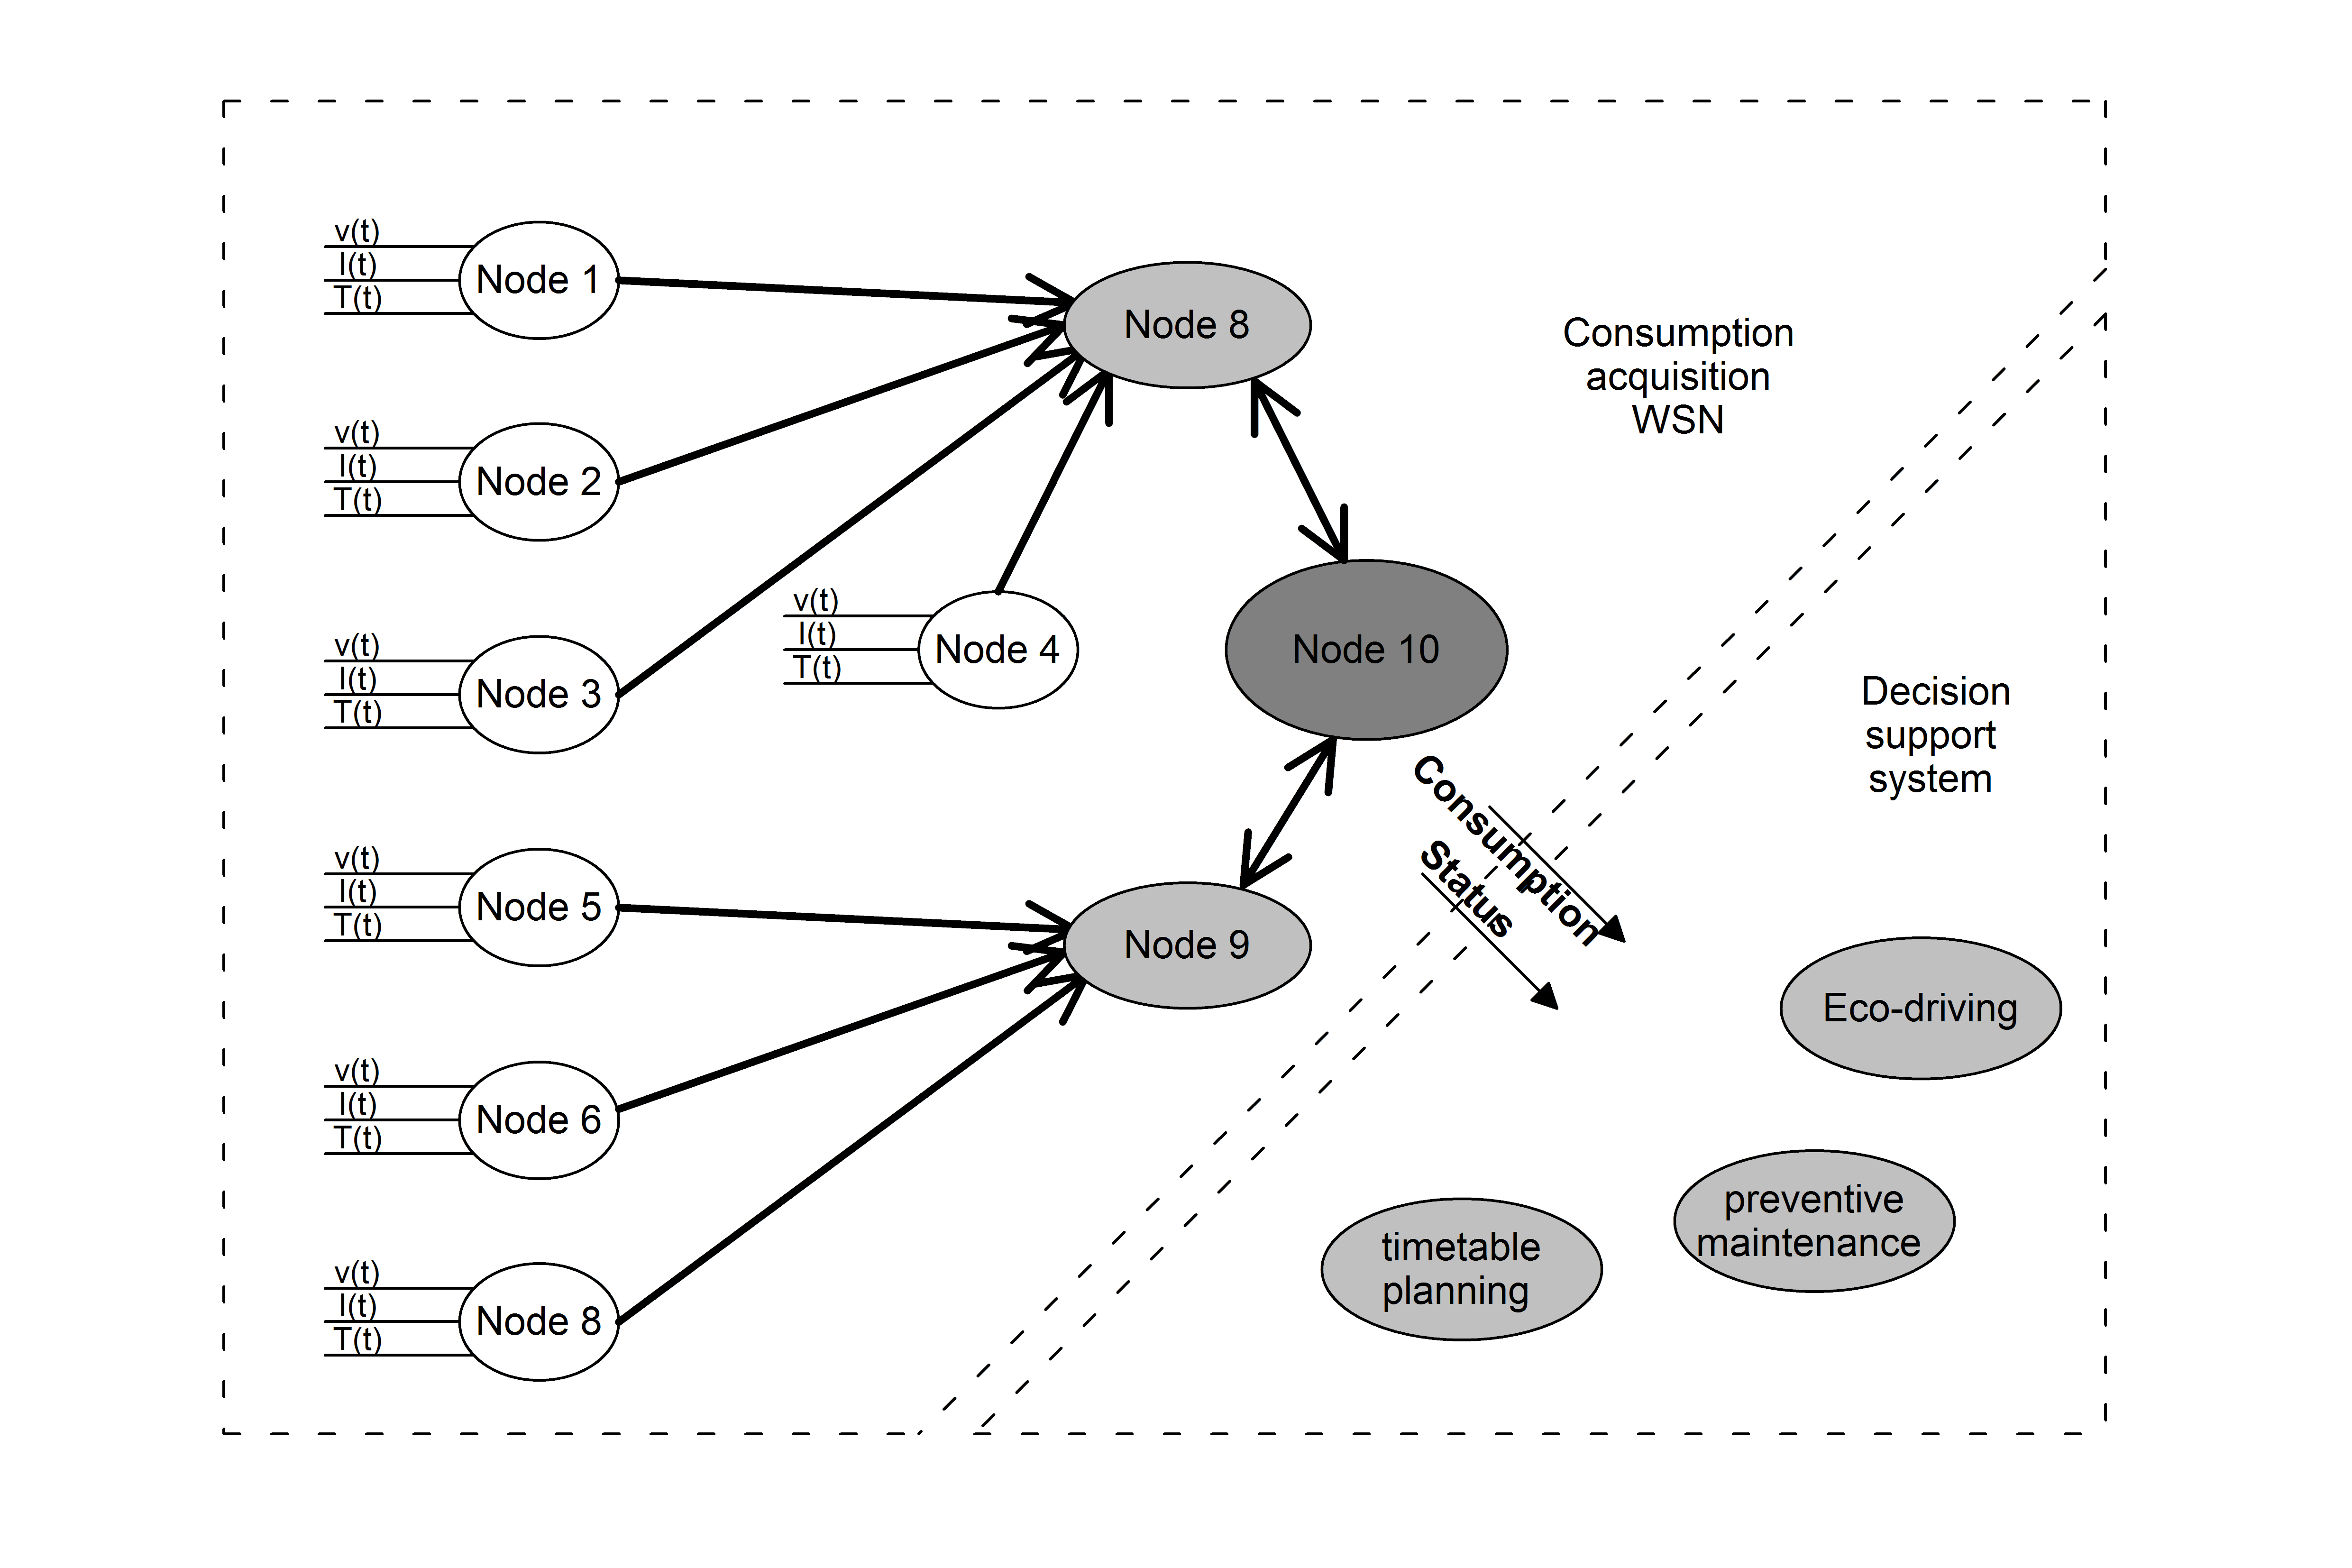
\includegraphics[width=0.75\textwidth,keepaspectratio]{figures/general}
	\caption{Integration of the WSN with a decision support system. }
	\label{fig:general}
\end{figure}

\newpage
Without an outlier detection mechanism, the decision support subsystem may have the following outputs:


\begin{description}
	\setlength\itemsep{-0.5em}
	\item[Input deviation from real value lower than a threshold]
	The Decision Support Subsystem output is in accordance to the real consumption conditions.
	\item[Input deviation from real value greater than a threshold]
	The Decision Support Subsystem output is not in accordance to the real consumption conditions.	
\end{description}

The problem of taking decisions based on wrong considerations of the consumption status is that it may lead to loss in desirable efficiency or increase of costs.

Let us consider a simple and hypothetical example where the DSS will provide an output towards suggesting an action in preventive maintenance based on the usage of a component. Considering that the usage of the component is depending on the counting of situations that the component is working above the nominal conditions. Without an outlier detection mechanism, the outliers will induce the DSS in counting situations of overcharge of the component, where the measurement is not related to working nominal conditions but is related to external influences, such as EMI or temperature. The output of DSS may suggest a preventive maintenance on a component that is working in proper conditions.

To conclude, with an outlier detection mechanism in the consumption acquisition subsystem the decision support subsystem may know if the value of consumption is an outlier or not and, with that information, the DSS output will be more accurate with the real conditions of operation.

%%%%%%%%%%%%%%%%%%%%%
%%   Wireless sensor networks
%%%%%%%%%%%%%%%%%%%%%
\newpage
\section{Outlier detection in WSNs}
\label{sec:od_wsn}
Wireless sensor networks (WSNs) has been widely used in several applications in several domains such as industrial, scientific, medical and others. Those applications have been supported by the advances in wireless technologies as well as in the evolution of microcontroller technologies, with enhanced processing capabilities associated with reduced energy consumption.

\subsection{Motivation}

\cite{class:rajasegarar:2007} points an important motivation for the inclusion of computational algorithms, i.e. outlier detection algorithms, to reduce the transmission of erroneous data, since in WSNs, the majority of the energy consumption occurs in radio communication. In particular, they present the case of Sensoria sensors and Berkeley motes, where the energy consumption in communication exceeds, in ranges from 1000 to 10000, the energy consumption of computation.

Thus, this raises a research opportunity to reduce the communication usage of $\mu C$s, by adding processing features, where the small increase in the computation will significantly reduce the energy consumption in the transmission. These processing features are, among others, the outlier detection algorithms.


On the field of the quality of the data acquired by WSNs, the motivation of detecting outliers in data acquired from WSNs has been extensively presented in the literature. The need for acquire data from harsh or "highly dynamic" environments as well as the need to validate and extract knowledge from the acquired data are one of the main points in the motivation to study the outlier detection in WSNs,  \cite{gen:zhang:2010,gen:chandola:2009,stat:ghorbel:2015,class:martins:2015b}.



\subsection{Research areas}
Zhang et al. \cite{gen:zhang:2010} identifies the outlier detection research areas in three domains: 

\begin{itemize}
	\item Intrusion detection: Situation caused by malicious attacks, where the detection techniques are query-driven techniques;
	
	\item Fault detection: Situation where the data suffer from noise and errors and where the detection techniques are data-driven ones;
	
	\item Event detection: Situation caused by the occurrence of one atomic or multiple events and where the majority of the research has been developed due to its complexity.
\end{itemize}

Based on the division of this three domains, the upcoming research is intended to be focused on the event detection and fault detection techniques. Specifically, the main goal for this research will be the event detection algorithms.


\subsection{Challenges}

The challenges of outlier detection in WSNs are related to the quality of the acquisition of the sensors, the reliability of the modules in terms of energy or environmental susceptibility, and the communication requirements and restrictions.

Zhang et al. \cite{gen:zhang:2010} lists the challenges as the following:

\begin{itemize}
	\setlength\itemsep{-0.5em}
	
	\item Resource constraints;
	
	\item High communication costs;
	
	\item Distributed streaming data;
	
	\item Dynamic network topology, \\ frequent communication failures, \\ mobility and heterogeneity of nodes;
	
	\item Large-scale deployment;
	
	\item Identifier outlier sources;
	
\end{itemize}

\cite{class:branch:2006} identifies an important challenge, where the probability of occurrence of outlier events are extremely small. \cite{nn:abid:2016} as well as \cite{stat:sheng:2007} identifies the large amount of data as the main challenge for outlier detection in WSN. \cite{nn:zhuang:2006} identifies the inexpensive and low fidelity sensors as the main reason for the error generation and the main challenge is identified on the distributed streaming data among a large amount of sensors. \cite{stat:ghorbel:2015} points the main challenge as the processing of data from sensors that generate continuously data, that is uncertain and unreliable. 

To conclude, the main challenge will be the usage of inexpensive and low fidelity sensors that will be affected by the rush railway environment. Complementary, the main challenge of using outlier detection mechanisms in the railway WSN is the balance between the detection accuracy and the influence that undetected data-instances will induce in other subsystems (in particular in decision support systems dependent on data from the WSN). In addition, the detection accuracy is directly related with the memory usage, computational requirements, communication overhead, etc. 


\newpage

\section{Classification of outlier}
\label{sec:classint}
\cite{gen:zhang:2010} presents aspects to be used as metrics  aimed to compare characteristics of different outlier detection techniques. In parallel, \cite{gen:chandola:2009} presents a similar approach for the classification of outlier detection. 
In table \ref{table:t1} is present a comparison between two approaches to classify the nature of input sensor data.

	
% Please add the following required packages to your document preamble:
% \usepackage{multirow}
\begin{table}[]
	\centering
	\caption{My caption}
	\label{my-label}

	\begin{tabular}{ llllll }
		\hline
		\multicolumn{3}{| c |}{Zhang et al.}                                                                                                                                                                          & \multicolumn{3}{ c |}{Chandola et al.}                                                                                                                                                                                                                                                                                                                                               \\ \hline
		\multicolumn{1}{|l}{\multirow{8}{*}{Input sensor data}} & \multirow{2}{*}{attributes}   & \multicolumn{1}{l|}{\multirow{2}{*}{univariate/multivariate}}                                                     & \multirow{8}{*}{Nature of input data} & \multirow{2}{*}{Described using attributes} & \multicolumn{1}{l|}{different types (binary, categorical, continuous)}                                                                                                                                                                                                                       \\ \cline{6-6} 
		\multicolumn{1}{|l}{}                                   &                               & \multicolumn{1}{l|}{}                                                                                             &                                       &                                             & \multicolumn{1}{l|}{quantity: i) univariate; ii) multivariate w/ same type; iii) multivariate w/ different data types;}                                                                                                                                                                      \\ \cline{2-3} \cline{5-6} 
		\multicolumn{1}{|l}{}                                   & \multirow{6}{*}{correlations} & \multicolumn{1}{l|}{dependencies among the attribures sensor nodes}                                               &                                       & \multirow{3}{*}{Related to each other}      & \multicolumn{1}{l|}{In sequence data, the data instances are linearlyordered, for example, time-series data, genome sequences, and protein sequences.}                                                                                                                                       \\ \cline{3-3} \cline{6-6} 
		\multicolumn{1}{|l}{}                                   &                               & \multicolumn{1}{l|}{\multirow{5}{*}{dependency of sensor node readings on history and neighboring node readings}} &                                       &                                             & \multicolumn{1}{l|}{In spatial data, each data instance is related to its neighboring instances, for example,vehicular traffic data, and ecological data. When the spatial data has a temporal (sequential) component it is referred to as spatio-temporal data, for example, climate data.} \\ \cline{6-6} 
		\multicolumn{1}{|l}{}                                   &                               & \multicolumn{1}{l|}{}                                                                                             &                                       &                                             & \multicolumn{1}{l|}{In graph data, data instances are represented as vertices in a graph and areconnected to other vertices with edges. Later in this section we will discuss situations where such relationships among data instances become relevant for anomalydetection.}                \\ \cline{5-6} 
		\multicolumn{1}{|l}{}                                   &                               & \multicolumn{1}{l|}{}                                                                                             &                                       & Relationship                                & \multicolumn{1}{l|}{Can be categorized based on relationship present among data instances}                                                                                                                                                                                                   \\ \cline{5-6} 
		\multicolumn{1}{|l}{}                                   &                               & \multicolumn{1}{l|}{}                                                                                             &                                       & \multirow{2}{*}{Applicability}              & \multicolumn{1}{l|}{for statistical techniques}                                                                                                                                                                                                                                              \\ \cline{6-6} 
		\multicolumn{1}{|l}{}                                   &                               & \multicolumn{1}{l|}{}                                                                                             &                                       &                                             & \multicolumn{1}{l|}{for nearest-neighbor-based techniques}                                                                                                                                                                                                                                   \\ \hline
		&                               &                                                                                                                   &                                       &                                             &                                                                                                                                                                                                                                                                                             
	\end{tabular}
\end{table}
	

Based on the work of \cite{gen:zhang:2010} and \cite{gen:chandola:2009}, the table \ref{table:t2} identifies the different types of outliers. 
Those types differ on the objective of the outlier detection techniques: detect anomalies in individual data instances or in groups of data to detect irregularities, respectively, in local or in the global measuring system.

% Please add the following required packages to your document preamble:
% \usepackage{multirow}
\begin{table}[h!]
	\centering
	\caption{Classification of the outlier techniques based on the type of the outlier/anomaly.}
	\label{table:t2}


\resizebox{1.0\textwidth}{!}{ 

	\begin{tabular}{c|c|c|c|c|c}
		\hline
		\multicolumn{3}{c|}{Zhang et al.}                                                                                                                                                                                                                                                                                                                                        & \multicolumn{3}{c|}{Chandola et al.}                                                                                                                                                                                                                                                                                                                                   \\ \hline
		\multicolumn{1}{|c|}{\multirow{6}{*}{\begin{tabular}[c]{@{}c@{}}Type\\ of\\ outliers\end{tabular}}} & \multirow{2}{*}{\begin{tabular}[c]{@{}c@{}}Local\\ outliers\end{tabular}}  & \begin{tabular}[c]{@{}c@{}}Variation 1:\\ anomalous values detection\\ only depends on its historical values\end{tabular}                                                             & \multirow{6}{*}{\begin{tabular}[c]{@{}c@{}}Type\\ of\\ anomaly\end{tabular}} & \multirow{2}{*}{\begin{tabular}[c]{@{}c@{}}Point\\ anomalies\end{tabular}}      & \multicolumn{1}{c|}{\multirow{2}{*}{\begin{tabular}[c]{@{}c@{}}An individual data instance\\ is considered anomalous,\\ with respect to the others\end{tabular}}}                                     \\ \cline{3-3}
		\multicolumn{1}{|c|}{}                                                                              &                                                                            & \begin{tabular}[c]{@{}c@{}}Variation 2;\\ anomalous values detection\\ depends on historical values\\ and on values of neighboring\end{tabular}                                       &                                                                              &                                                                                 & \multicolumn{1}{c|}{}                                                                                                                                                                                 \\ \cline{2-3} \cline{5-6} 
		\multicolumn{1}{|c|}{}                                                                              & \multirow{3}{*}{\begin{tabular}[c]{@{}c@{}}Global\\ outliers\end{tabular}} & \begin{tabular}[c]{@{}c@{}}Variation 1:\\ All data is transmitted\\ to a centralized architecture\\ where outlier detection \\ techniques takes place\end{tabular}                    &                                                                              & \multirow{3}{*}{\begin{tabular}[c]{@{}c@{}}Contextual\\ anomalies\end{tabular}} & \multicolumn{1}{c|}{\begin{tabular}[c]{@{}c@{}}Contextual attributes:\\ are used to determine \\ the context for a given instance\end{tabular}}                                                       \\ \cline{3-3} \cline{6-6} 
		\multicolumn{1}{|c|}{}                                                                              &                                                                            & \begin{tabular}[c]{@{}c@{}}Variation 2:\\ Data from a cluster of sensors\\ is used for outlier detection\\ in a aggregate/clustering\\  based architecture\end{tabular}               &                                                                              &                                                                                 & \multicolumn{1}{c|}{\multirow{2}{*}{\begin{tabular}[c]{@{}c@{}}Behavioral attributes:\\ defines the noncontextual \\ characteristics of a \\ given instance.\end{tabular}}}                           \\ \cline{3-3}
		\multicolumn{1}{|c|}{}                                                                              &                                                                            & \begin{tabular}[c]{@{}c@{}}Variation 3:\\ Individual nodes can identify\\ global outliers if they have\\  a copy of global estimator model\\ obtained from the sink node\end{tabular} &                                                                              &                                                                                 & \multicolumn{1}{c|}{}                                                                                                                                                                                 \\ \cline{2-3} \cline{5-6} 
		\multicolumn{1}{|c|}{}                                                                              & \multicolumn{2}{c|}{}                                                                                                                                                                                                                                              &                                                                              & \begin{tabular}[c]{@{}c@{}}Collective\\ anomalies\end{tabular}                  & \multicolumn{1}{c|}{\begin{tabular}[c]{@{}c@{}}If a collection of related data\\ instances is anomalous\\ with respect to the entire data set,\\ it is defined as a collective anomaly.\end{tabular}} \\ \hline
	\end{tabular}

}
\end{table}

\newpage


Table \ref{table:t3} continues the classification, focusing in three parts: 
\begin{itemize}
		\setlength\itemsep{-0.5em}
		\item The need of pre-classified data (to implement supervised, semi-supervised or unsupervised outlier detection techniques);
		
		\item The output of outlier detection techniques (binary labels for normal/abnormal data-set and a score for each data-set to evaluate the weight of being an anomaly)
		
		\item The identity of the outliers (detect errors, events or malicious attacks)
\end{itemize}

\newpage

% Please add the following required packages to your document preamble:
% \usepackage{multirow}
\begin{table}[h!]
\centering
\caption{ Classification of outlier detection techniques according to: i) need of pre-classified data; ii) output of detection techniques; iii) identity of outliers}
\label{table:t3}


\resizebox{1.0\textwidth}{!}{ 
	
\begin{tabular}{c|c|c|c|c|c}
	\hline
	\multicolumn{3}{c|}{Zhang et al.}                                                                                                                                                                                                                                                                                     & \multicolumn{3}{c|}{Chandola et al.}                                                                                                                                                                                                                                                                                                                                             \\ \hline
	\multicolumn{1}{|c|}{\multirow{3}{*}{\begin{tabular}[c]{@{}c@{}}Availability\\ of\\ pre-defined\\ data\end{tabular}}} & Supervised                                                  & \begin{tabular}[c]{@{}c@{}}Require pre-classified\\ normal and abnormal data\end{tabular}                                       & \multirow{3}{*}{\begin{tabular}[c]{@{}c@{}}Data\\ labels:\\ normal or\\ anomalous\end{tabular}} & \begin{tabular}[c]{@{}c@{}}Labels obtained by\\ Supervised\\ Anomaly Detection\end{tabular}       & \multicolumn{1}{c|}{\begin{tabular}[c]{@{}c@{}}Training data has labeled instances \\ for normal and anomalous classes\end{tabular}}                                       \\ \cline{2-3} \cline{5-6} 
	\multicolumn{1}{|c|}{}                                                                                                & Semi-supervised                                             & \begin{tabular}[c]{@{}c@{}}Require only pre-classified\\ normal data\end{tabular}                                               &                                                                                                 & \begin{tabular}[c]{@{}c@{}}Labels obtained by\\ Semi-supervised \\ Anomaly Detection\end{tabular} & \multicolumn{1}{c|}{\begin{tabular}[c]{@{}c@{}}Training data has labeled instances\\ only for normal class.\\ There is no labels for the\\ anomalous classes\end{tabular}} \\ \cline{2-3} \cline{5-6} 
	\multicolumn{1}{|c|}{}                                                                                                & Unsupervised                                                & Do not require pre-classified data                                                                                              &                                                                                                 & \begin{tabular}[c]{@{}c@{}}Labels obtained by\\ Unsupervised\\ Anomaly Detection\end{tabular}     & \multicolumn{1}{c|}{\begin{tabular}[c]{@{}c@{}}Techniques that do not require\\ training data\end{tabular}}                                                                \\ \hline
	\multicolumn{1}{|c|}{\multirow{2}{*}{\begin{tabular}[c]{@{}c@{}}Degree of\\ being an \\ outlier\end{tabular}}}        & Scalar                                                      & \begin{tabular}[c]{@{}c@{}}Zero-one classification:\\ Classifies a data measurement\\ into normal or outlier class\end{tabular} & \multirow{5}{*}{\begin{tabular}[c]{@{}c@{}}Output\\ of\\ Anomaly\\ detection\end{tabular}}      & \multirow{2}{*}{Scores}                                                                           & \multicolumn{1}{c|}{\multirow{2}{*}{\begin{tabular}[c]{@{}c@{}}Degree of which a data instance\\ is consider an anomaly\end{tabular}}}                                     \\ \cline{2-3}
	\multicolumn{1}{|c|}{}                                                                                                & Score                                                       & \begin{tabular}[c]{@{}c@{}}Assign to each data measurements\\ a outlier score;\\ Display a ranked list of outliers\end{tabular} &                                                                                                 &                                                                                                   & \multicolumn{1}{c|}{}                                                                                                                                                      \\ \cline{1-3} \cline{5-6} 
	\multicolumn{1}{|c|}{\multirow{3}{*}{\begin{tabular}[c]{@{}c@{}}Identity\\ of\\ outliers\end{tabular}}}               & Errors                                                      & \begin{tabular}[c]{@{}c@{}}Noise-related measurement\\ or data coming from a faulty sensor\end{tabular}                         &                                                                                                 & \multirow{3}{*}{Labels}                                                                           & \multicolumn{1}{c|}{\multirow{3}{*}{\begin{tabular}[c]{@{}c@{}}Provide binary labels\\ (normal/anomalous)\end{tabular}}}                                                   \\ \cline{2-3}
	\multicolumn{1}{|c|}{}                                                                                                & Events                                                      & \begin{tabular}[c]{@{}c@{}}Particular phenomena\\ that changes the real-world state\end{tabular}                                &                                                                                                 &                                                                                                   & \multicolumn{1}{c|}{}                                                                                                                                                      \\ \cline{2-3}
	\multicolumn{1}{|c|}{}                                                                                                & \begin{tabular}[c]{@{}c@{}}Malicious\\ attacks\end{tabular} & \begin{tabular}[c]{@{}c@{}}Related to network security issues \\ (Outside of the scope of the paper)\end{tabular}                               &                                                                                                 &                                                                                                   & \multicolumn{1}{c|}{}                                                                                                                                                      \\ \hline
\end{tabular}

}

\end{table}

\vspace{2em}



\section{Taxonomy of Outlier Detection Techniques}
\label{sec:taxon}
The study of detection techniques requires a well-defined taxonomy framework that addresses the related work on the different areas. This taxonomy is well defined and solid in the literature, where the works of \cite{gen:zhang:2010} and \cite{gen:chandola:2009} reflect a similar approach on presenting a taxonomy for outlier detection techniques.

In the following sections, a coverage in relevant techniques is presented:

\begin{itemize}
	\setlength\itemsep{-0.5em}
	\item Classification based techniques.
	\subitem Bayesian Networks
	\subitem Rule-based techniques
	\subitem Support Vector Machines
	
	\item Statistical based techniques.
	\subitem Parametric --- Gaussian based
	\subitem Non-parametric --- Histogram based
	\subitem Non-parametric --- Kernel function based
	
	\item Nearest Neighbor-based techniques.
	\subitem Using distance
	\subitem Using relative density
	
	\item Clustering based techniques.
	
	\item Spectral Decomposition based techniques.
	
\end{itemize}


%%%o resto deste capítulo está dividido em ficheiros












\newpage

\section{Classification based techniques}

Classification based techniques are based on systematic learning approaches based on sets of data. 
The supervised approaches requires knowledge to train a model (or classifier) from a set of data instances (or training data) and classifies a new data instance as normal or as outlier. 
The unsupervised approaches do not require knowledge and learn the boundary around normal instances, declaring the new instance as normal or as outlier depending if the data instance is outside of the boundary of the previous data sets.

The classification based techniques are listed as the following:

\begin{itemize}
	\setlength\itemsep{-0.5em}
	\item Neural Networks-based;
	\item Bayesian Networks-based;
	\item Rule-based;
	\item Support Vector Machines-based.
	
\end{itemize}

Neural networks-based approaches are interesting strategies for outlier detection where a given neural network might be trained with only normal data-sets. 
At testing stage, the data instances that are similar to the training data-set are accepted by the neural network and then considered as normal. 
The remaining data-sets are rejected by the neural network due to their lack of similarity with normal data-sets. Thus, those data instances are considered as outliers. 
Based on the table \ref{table:t3}, these techniques are classified as semi-supervised due to their need for normal data-sets for the training stage.

Bayesian networks-based approaches are identified as prominent techniques for outlier detection in WSNs, being the reason why they are extensively covered further on.
Those techniques ...

Rule based ...

Support Vector Machine (SVM) relies on ...

\subsection{Bayesian Networks}

Zhang et al. <zhang2010> divide the bayesian network based techniques in three categories: 

\begin{itemize}
	\setlength\itemsep{-0.5em}
	\item Na\"{i}ve Bayesian Networks;
	\item Bayesian Belief Networks;
	\item Dynamic Bayesian Network Models;	
\end{itemize}

All those approaches uses probabilistic graphical models to represent a set of variables and their probabilistic interdependencies. 
This graphical model aggregates the information from different variables and provides an estimate on the expectancy of an event to belong to the learned class.

Xiang et al. <xiang2015> illustrates an application to measure the concentration of NO$_2$, CO and O$_3$ pollutants, using a bayesian network. All the three variables are all correlated and also depends on the temperature as presented in figure \ref{fig:xiang2016}. The real measurements acquired by the microcontroller are represented with (s) and the representations in (t) refers to the real concentration of those pollutants.

\begin{figure}[h!]
	\centering
	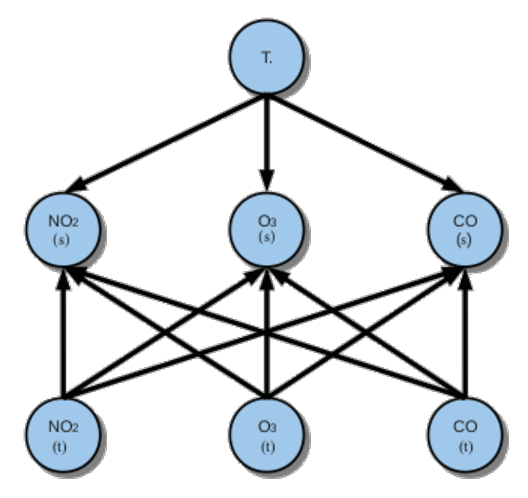
\includegraphics[width=0.60\textwidth,keepaspectratio]{figures/xiang2016}
	\caption{Application of a Bayesian Network to an atmospheric measurement system. }
	\label{fig:xiang2016}
\end{figure}

The three categories presented by Zhang et al. differs between them where the first category captures the sensor nodes correlations on spatio-temporal domain; 
The second one considers not only the spatio-temporal correlations but also the conditional dependence of sensor attributes;
The third category proposes the measurement of state variables at a current time instance.

Janakiram et al. <janakiram2006> proposes the detection of outliers in sensor streamed data by capturing the conditional dependencies among the observation of it's attributes. this is made in three phases:

\begin{description}
	\setlength\itemsep{-0.5em}
	\item[Training Phase]  
	Phase where the Bayesian Belief Network is trained to capture the spatio-temporal correlations.
	\item[Testing Phase]  
	Phase where the trained BBN is tested on the level of accuracy and, if needed, the learned parameters are updated.
	\item[Inference Phase] 
	Phase where the missing values are inferred and the remaining streamed data are tested to detect if it is an outlier or not.
\end{description}

Janakiram et al. also defined the BBN, where the BBN is a directed graph, together with an associated set of probabilistic tables.
The graph is divided in nodes and arcs, where the nodes represents the variables and the arcs are the representation of the casual/influential relationship among variables.

The main contribution of BBN is the possibility to have a model that, with the dependency between uncertain variables (by filling a node probability table), it is possible to describe complex probabilistic reasoning about uncertainty.

Janakriam et al. describes their process in three steps:

\begin{itemize}
	%\setlength\itemsep{-0.5em}
	
	\item Constructing the Bayesian Belief Network
	\subitem \textbf{IF} a few variables have direct dependencies
	\subitem \textbf{AND} many of the variables are conditionaly independent
	\subitem \textbf{THEN} all the probabilities can be computed from the joint probability distribution.
	
	\item Learning Bayesian Belief Networks
	\subitem \textbf{IF} the network structure is given
	\subitem \textbf{AND} all variables are fully observable in the training examples
	\subitem \textbf{THEN} estimating the conditional probabilities is enough
	\subitem
	\subitem \textbf{IF} the network structure is given
	\subitem \textbf{AND} some of the variables are observable
	\subitem \textbf{THEN} apply neural network using Gradient Ascent Procedure
	\subitem
	\subitem \textbf{IF} the network structure is unknown
	\subitem \textbf{THEN} Use heuristic search
	\subitem \textbf{OR} Use constraint-based technique to search through potential structures
	
	
	\item Inferring from Bayesian Belief Networks
	\subitem \textbf{THESIS} The probability distribution of certain attributes might be inferred
	\subitem \textbf{PROOF} Given the fact that the values that other attributes can take are known	
\end{itemize}

Paola et al <paola2014> proposes an adaptive distributed Bayesian approach for detecting outliers in data collected by a WSN.
The focus of the proposed algorithm is the optimization of outlier classification accuracy, time and communication complexity and also considering externally imposed constraints on conflicting goals. The proposed algorithm is intended to run in each sensor node. 

From the individual sensor node point of view, this algorithm consists in two phases:

\begin{description}
	\setlength\itemsep{-0.5em}
	\item[Outlier detection]  
	Where, based on sensor readings and on the collaboration with neighbors, is made the probabilistic inference where the results are evaluated in three metrics: classification accuracy, time complexity and communication complexity.
	
	\item[Neighborhood selection] 
	Where the best neighbors are identified ad selected to cooperate with, and, in addiction, to correspond to a reconfiguration of the Bayesian Network structure.
\end{description}

In the global point of view, if there is a high number of cooperating nodes, the classification is naturally higher with the drawback if increasing the processing time and communication complexity (thus resulting in increased detection delay and increase of energy consumption).

Xiang et al. <xiang2016> proposes the addition of recover and recalibrate the drifted sensors simultaneously based on the usage of a Bayesian network.

The authors have applied their algorithm to the measurement of the variables in the sensor readings of the NO$_2$, CO and O$_3$ pollutants, as previously presented in figure \ref{fig:xiang2016}.
Based on the correlations of the sensor readings and on the temperature influence, the algorithm itself detects the outliers, recover valid information and adjust the BBN to automatically recalibrate the sensor.




\subsection{Rule-based techniques}

Rule based is another classification based technique for outlier detection. Similarly, this technique is based on a training stage from a data-set and a model generation to detect new data-instances based on history values.

Rule based techniques depends on two steps <chandola2009>:

\begin{itemize}
	%\setlength\itemsep{-0.5em}
	\item \textbf{Learn rules from the training data-set}\\
	Using a learning algorithm (i.e. RIPPER, Decision Tree, etc.)\\
	Where each rule has an associated confidence value 	proportional to the ratio:\\
	{\centering	$\text{\footnotesize Confidence Value} = \frac{\text{number of training instances correctly classified by the rule}}{\text{number of total training instances covered by the rule}}$
}
		
	\item \textbf{Find for each test instance the rule}\\
	That better capture the given test instance.
	
	\item \textbf{The anomaly score is}\\
	The inverse of the confidence value for the rule that better capture the test instance.

\end{itemize}

Islam et al. 2016 <islam2016> proposes an algorithm for outlier detection inserted in rule-based taxonomy. They propose a new belief-rule-based association rule, with the focus on handling various types of uncertainties. 

Due to the nature of the sensor data, a traditional inference mechanism can not be used. Therefore they propose a new inference mechanism for the rule-based algorithm that consists of an input transaction databased that is converted into the following:
\begin{itemize}
	\setlength\itemsep{-0.5em}
	\item belief transaction database;
	\item support calculation;
	\item belief matrix;
	\item confidence calculation;
	\item belief association rule discovery.
	
\end{itemize}


\newpage

\subsection{Support Vector Machines}

Rather than performing outlier detection in the central node, Rajasegarar et al. <rajasegarar2007> proposes a 
distributed approach to:

\begin{itemize}
	\setlength\itemsep{-0.5em}
	\item performs detection on local data at each node
	\item and communicates only the summary information to perform the global classification of the data.	
\end{itemize}

Their proposal is based on a one-class quarter sphere svm and is divided into 2 parts:

\begin{itemize}
	\setlength\itemsep{-0.5em}
	\item \textbf{Anomaly detection  algorithm}
	\subitem The OD is supported by previous works where, with the fitness approach of a hypersphere to the data in a higher dimensional space, and by applying a linear optimization to the problem of fitting the hypersphere with minimal radius R, having the center fixed at the origin and encompassing the majority of the image vectors.
	\subitem The result of the linear optimization problem is the classification of the image vectors as:
	\subitem  \textbf{$\rightarrow$ Support Vectors}, if inside the sphere;
	\subitem  \textbf{$\rightarrow$ Outliers}, otherwise.
	
	\item \textbf{Distributed anomaly detection}
	\subitem 1. Each sensor node runs the entire AD algorithm on local data;
	\subitem 2. The resulting radius is sent to the parent node;
	\subitem 3. Each parent computes the global radius;
	\subitem 4. Parents sends the radius to children nodes;
	\subitem 5. Children compares global radius with local one and updates parameters.
		
\end{itemize}


Xu et al. 2012 <xu2012> proposes a KNN-SVM which is a Support Vector Machine based on K-Nearest Neighbor Algorithm.

Despite KNN taxonomy is presented further on in section 3.7, in a synthesis  the KNN is a distance-based approach that detect outliers in adata-instances lying in the sparsest regions or lying in the outside of a given model boundary of the feature space.

Considering the Quarter sphere SVM technique proposed by Rajasegarar et al. or by Sun et al 2008 <sun2008> the KNN-SVM combine the origin and the radius R that contain most of the samples and introduces kernel functions to make the optimization region more tighten.

Martins et al.<martins2015a, martins 2015b> has proposed a modifies SVM based on a kernel-based technique. In parallel, they propose an online sliding window scheme. The modification extends the original LS-SVM to be applied to the transient raw data collected from transmitters attached to a WSN. In a posterior work, Gil et al. <gil2016> compares the LS-SVM with PCA (a technique that will be presented further on in section 3.9).
\newpage






\newpage

\section{Statistical based techniques}
\label{sec:statbased}
\subsection{Parametric --- Gaussian based}
\subsection{Non-parametric --- Histogram based}
\subsection{Non-parametric --- Kernel function based}

\section{Nearest Neighbor-based techniques}
\subsection{Using distance}
\subsection{Using relative density}
\newpage


\section{Clustering based techniques}
\label{sec:clustbased}
%\lipsum[4-4]

\cite{gen:chandola:2009} synthesizes the clustering techniques in three categories based on three different assumptions: 

\begin{itemize}
	
	\setlength\itemsep{-0.5em}
	
	\item The normal data instances are part of a cluster in the data and the outliers does not fit any cluster;
	
	\item The normal data instances are present close to it's closest cluster centroid and the outliers lies far way from their closest cluster centroid;
	
	\item The normal data instances are part of large dense clusters and the outliers are part of small or sparse clusters.
	
\end{itemize}

\cite{clust:rajasegarar:2006} uses a technique to minimize the communication overhead by using clusters among the sensor readings. In a further step, it merges the clusters before the data is sent to other nodes.


\section{Spectral Decomposition based techniques}




\chapter{Future Research}
%\lipsum[4-4]
In this chapter there are presented the future steps in research on outliers detection on railways WSN-based smart grid.


%%%%%%%%%%%%%%%%%%%%%
%%   Smart metering Systems
%%%%%%%%%%%%%%%%%%%%%
\section{Evaluation of effect of undetected outliers in railway WSN}


During the state of the art, the definition of "what is an outlier in railways WSN" was slightly covered, resulting in raising the research question:

\fbox{
	\centering
	\textbf{What is the effect of an undetected outlier in an railways WSN?}
} 

A railways WSN is focused on acquiring the data (in forms of measurements) from the railways environment with the purpose of providing that information to a subsystem (such as a decision support system). Having this in mind, an assumption should be made to define the outlier as the effect of erroneous information retrieved from the DSS due to erroneous data from the measurement. A major contribution of an outlier detection mechanism is the validation of the quality of the output of the DSS. In particular, if a measurement or a set of measurements are detected as outliers, the DSS will have the information of the quality of his output, as is shown in figure \ref{fig:evaluation}.

\begin{figure}[h!]
	\centering
	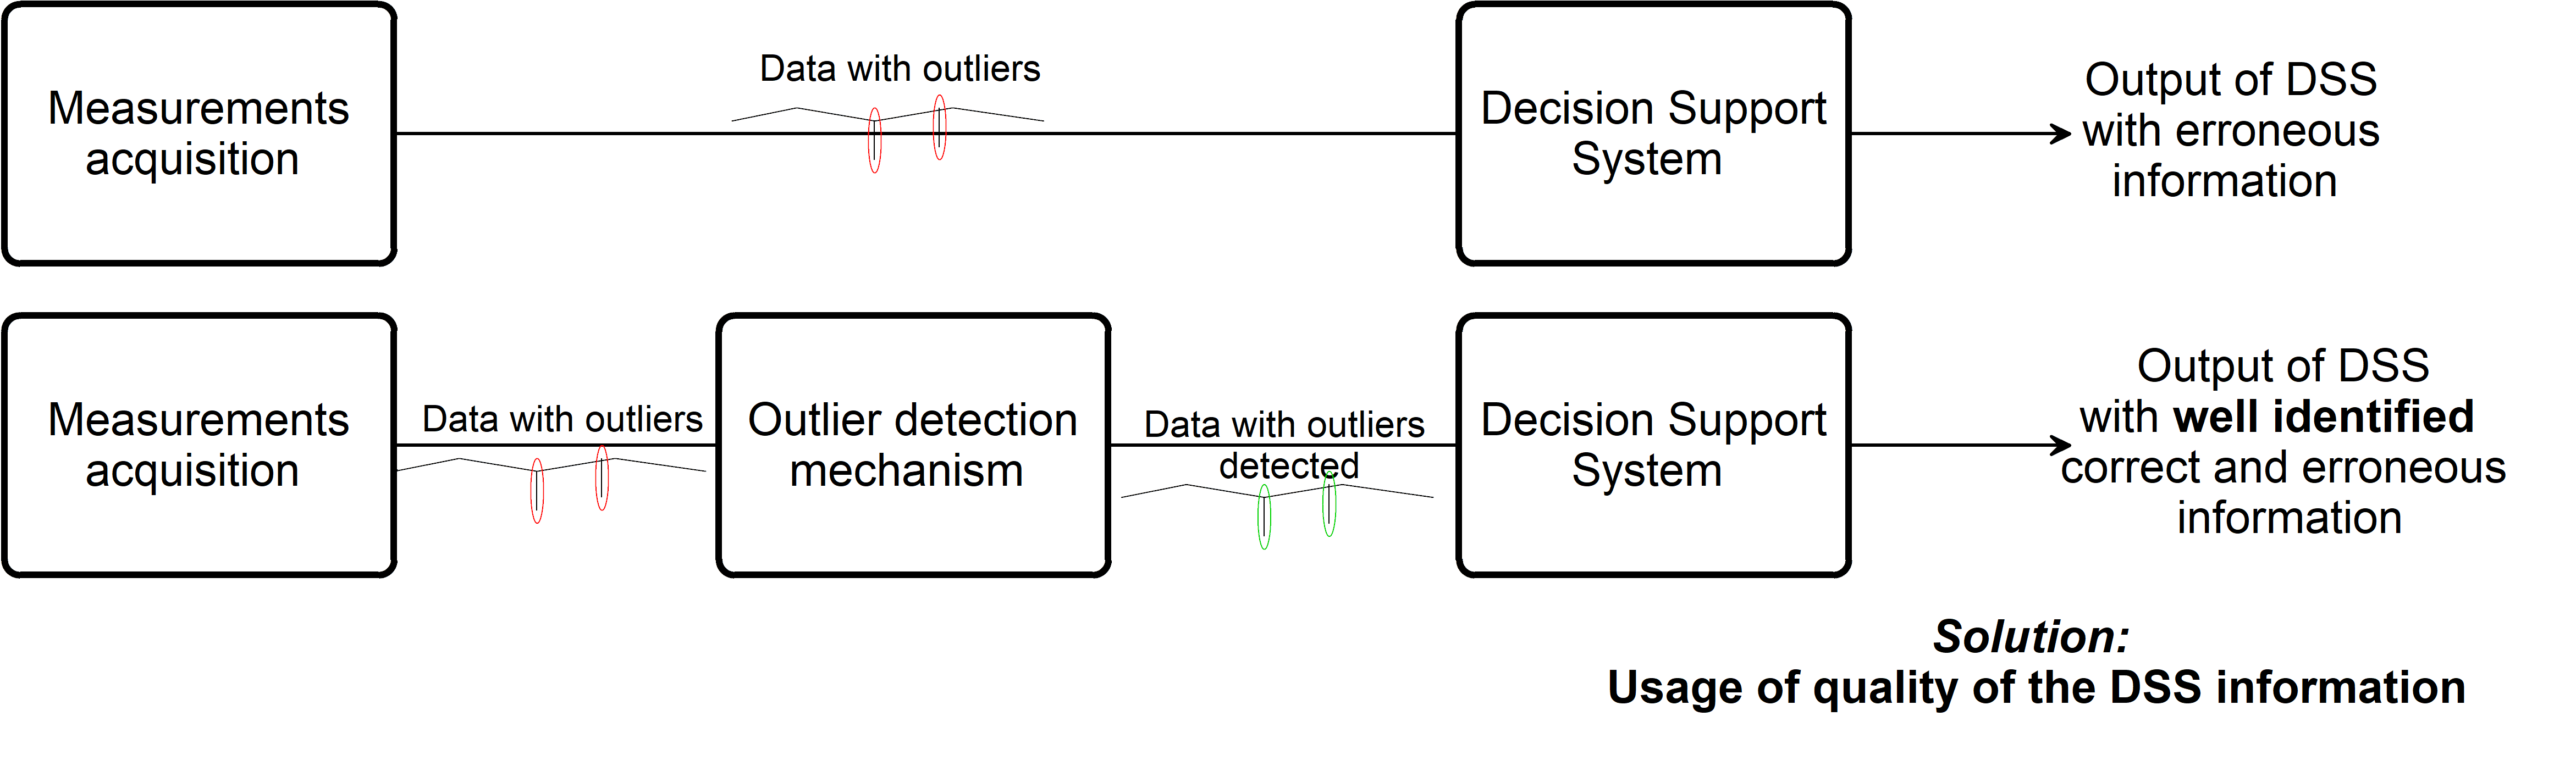
\includegraphics[width=1.03\textwidth,keepaspectratio]{figures/evaluation}
	\caption{Comparison of the output of DSS with and without an outlier detection mechanism. }
	\label{fig:evaluation}
\end{figure}

It is important at this moment to present examples of DSS. Eco-driving strategies and timetable planning require conservative measurements of energy consumption in several points of the railway electrical system, where the situations of outliers should result, in example, in default outputs of DSS; On other side, preventive maintenance may find resourceful the presence of outliers considering that those outliers reflect anomalous behavior due to unknown external effects (on the measurement).

The methodology will embrace the simulation of the railway WSN system. With a well defined simulation model that mimics the behavior of the DSS, the measurements acquisition system and the wireless network, the effect of undetected outlier can be evaluated before and after the DSS.

Considering the literature, two possibilities will be considered as a starting point for this railway WSN system simulator: the NS-3 and the contiki-cooja network simulators. However, for the future research, a higher analysis on the available simulators must be considered.


\section{Selection of Outlier detection mechanism}

On the previous section, the need of a simulation model was presented. However, based on real data from railway systems (or similar) can validate the implementation of an outlier detection mechanism.

In this way, a set of outlier detection mechanisms can be validated with a given testbench. The research question that can be raised is the following:\textbf{What is the effect of an undetected outlier in an railways WSN?}




\chapter{Conclusion}


This work presents the study of outlier detection techniques, covering the state of the art and focusing the study towards the implementation of those techniques in a railways remote monitoring system.

In the perspective of fault-tolerance in computing systems domain, those techniques are of extreme interest to avoid the unwanted failures in computing systems.
Following the taxonomy extensively presented in the literature, an outlier is considered as a fault in the input of the system. This fault will be a cause of an error and, without a outlier detection mechanism, those errors can be propagated to the outer frontier of the system, resulting on failure, or in a better definition, resulting in a behavior that is not according to the specifications. 
The task of those techniques is to detect the outliers in the computing system and avoid them to be propagated to the output of the system. 

Based on this domain of fault-tolerance in computing systems, the definition of frontier of the railways WSN was proposed. In particular, the railways remote monitoring system as previously presented, provides data and information for a Decision Support System (DSS).
Rather than considering only the data provided from the sensor network, an important step is to evaluate and avoid failures in the entire system (constituted by the sensing subsystem - that collects the data from the environment - and the DSS subsystem - that generates decision information based on the available data). 

As a starting point for future research, with this work two research questions was presented towards deepen this domain. An iterative procedure is expected to be taken by continuously searching in the literature for new improvements on this domain and continuous to deepen towards an new contribution. At this moment, a methodology is presented for the immediate future to implement an outlier detection technique in a energy monitoring test-bench.




%\bibliography{outliers,references}
%\bibliography{outliers}
\PrintBib{outliers}


%\bibliographystyle{plainnat}
%\bibliography{references}


\end{document}